\documentclass[UTF8]{EPURapport}
%\usepackage{listings}

%\renewcommand{\lstlistlistingname}{Liste des codes}
%\renewcommand{\lstlistingname}{Code}

%\addextratables{%
%	\lstlistoflistings
%}

%\swapAuthorsAndSupervisors

\thedocument{Cahier d'analyse}{Canne connectée pour aveugles}{}
\grade{Département Informatique\\ 5\ieme{} année\\ 2020-2021}
\authors{%
	\category{Auteurs}{%
		\name{Djawad M'DALLAH MARI} \mail{djawad.mdallah-mari@etu.univ-tours.fr}
	}
	\details{DII5 2020-2021}
}
\supervisors{%
	\category{Encadrants}{%
		\name{Gilles VENTURINI} \mail{gilles.venturini@etu.univ-tours.fr}
	}
	\details{Université François-Rabelais, Tours}
}
\abstracts{Cahier d'analyse canne connecée pour aveugles}
{}
{}
{}

\begin{document}

\chapter{Cahier d'analyse}

\section{Introduction}
Ce cahier d'analyse s'inscrit dans le cadre du projet Canne connectée pour aveugles. Il vise à présenter les analyses faites pour répondre aux besoins exprimés dans le cahier de spécifications. Une lecture au préalable du cahier de spécifications est donc recommandée afin de comprendre le contexte et les enjeux du projet.

Nous verrons donc dans ce document une analyse sur l'application Android à développer. Nous verrons en particulier quelques méthodes de reconnaissances d'objet pour le mobile, les différentes méthodes qui permettront d'informer l'utilisateur et également comment garantir à l'utilisateur une interface adaptée à ses contraintes.

\section{Reconnaissance d'objet}
\subsection{Librairies}
L'un des besoins primaires pour la réalisation de ce projet est la reconnaissance d'objet. Pour cela, il est important de choisir une librairie qui permet d'implémenter un réseau de neurones. Sur Android il existe l'Android Neural Networks API (NNAPI) qui est un API en C permettant de réaliser des opérations de machine learning. Il a été conçu pour fournir une couche de fonctionnalités bas niveau qui sera ensuite utilisable par des couches plus hauts niveau comme les frameworks TensorFlow ou encore Caffe2. Toutefois, il est tout à fait possible de faire abstraction des frameworks et implémenter une solution utilisant directement l'API. L'utilisation la plus commune est avec TensorFlow et plus précisément TensorFlow Lite qui est une version allégée de TensorFlow. Cette version allégée limite certaines opérations de TensorFlow lui permettant donc d'être utilisée pour les appareils embarqués. Il existe également Keras, un autre outil intéressant permettant de faire du machine learning. Cependant, dès lors que l'on souhaite déployer sur Android, il faudra passer par TensorFlow Lite et convertir le modèle en format TensorFlow Lite \footnote{\url{https://keras.io} : partie "Deploy Anywhere."}. Dans notre cas, l'utilisation de TensorFlow Lite pourrait suffire pour répondre à notre besoin. De plus, celle-ci dispose d'un large panel de modèles préentrainés comme on va le voir dans les parties qui suivent.  

\subsection{Modèles}
Un modèle est un fichier qui a été entraîné pour reconnaître certains types de motifs (pattern). Il est entraîné à partir d'un ensemble de données et utilise un algorithme qui lui permet "d'apprendre" à travers ces données. \\

Le choix du bon modèle est un facteur important pour répondre au besoin de reconnaissance d'objet. En effet, toute l’application, pour qu'elle soit utile aux utilisateurs finals, dépend de la capacité du modèle à détecter et identifier un objet. Afin de répondre à ce besoin, il faudrait faire un inventaire des modèles de reconnaissance d'objet disponible puis faire des comparaisons. Pour mesurer les performances de chaque modèle, des critères doivent être établis (latence, disponibilité, rapidité, coût, ...) ainsi que des conditions de fonctionnement bien définis (caractéristique du smartphone, version d'Android, version, ...). Cela permettrait d'avoir un environnement d'exécution commun pour chaque modèle et donc des mesures cohérentes.

\subsubsection{Modèles disponibles}
Avec la librairie TensorFlow, nous disposons d'un grand panel de modèles préentrainés. La plupart de ces modèles ne sont pas directement compatible avec TensorFlow Lite. Ceux sur TF2 Detection Zoo \footnote{\url{https://github.com/tensorflow/models/blob/master/research/object_detection/g3doc/tf2_detection_zoo.md}} peuvent être convertis en utilisant TFLite Converter \footnote{\url{https://www.tensorflow.org/lite/convert}}. Les modèles déjà adaptés TensorFlow Lite sont disponibles sur le hub officiel de TensorFlow, mais peu de modèles de reconnaissance d'image y sont rescencés notamment de reconnaissance d'objets (\textbf{Object Detection}) \footnote{\url{https://tfhub.dev/s?deployment-format=lite&module-type=image-object-detection}}. En effet, il existe que trois modèles officiels dans cette catégorie : SSD MobileNet, Mobile Object Localizer et East Text Detector. Parmi ces trois modèles, on peut déjà abandonner le East Text Detector puisqu'il s'agit ici de détecter du texte. En revanche, d'autres modèles de reconnaissance d'objet sont disponibles sur le github de TensorFlow \footnote{\url{https://github.com/tensorflow/models/blob/master/research/object_detection/g3doc/tf1_detection_zoo.md}} mais devront également être converti en mobile pour pouvoir être utilisés sur Android. Ces modèles là sont intéressants car ils n'ont pas tous la même architecture de réseau de neuronnes (CenterNet, EfficientNet, Faster R-CNN, ...), on pourra donc choisir celui qui répond le plus à notre besoin (voir partie \ref{choixmodele} Choix du modèle). Au niveau des modèles de \textbf{Classification}, il existe un peu plus de modèles compatibles TensorFlow Lite \footnote{\url{https://tfhub.dev/s?deployment-format=lite&module-type=image-classification}}. Les modèles de classification, malgré le fait qu'ils sont plus précis, vont moins répondre à notre besoin initial, mais méritent d'être évoqués puisque ceux-ci pourrait être mis en place dans une version future du projet ; en complément du modèle de reconnaissance d'objet choisi par exemple.

\subsubsection{Object Detection vs Classification}
Les modèles de reconnaissances d'objet (\textbf{Objet Detection}) sont capables de localiser et identifier plusieurs objets sur une même image, tandis que les modèles de \textbf{Classification} ne détecte qu'un seul objet sur une image.
\newpage

\begin{figure}[h!]
\centering
  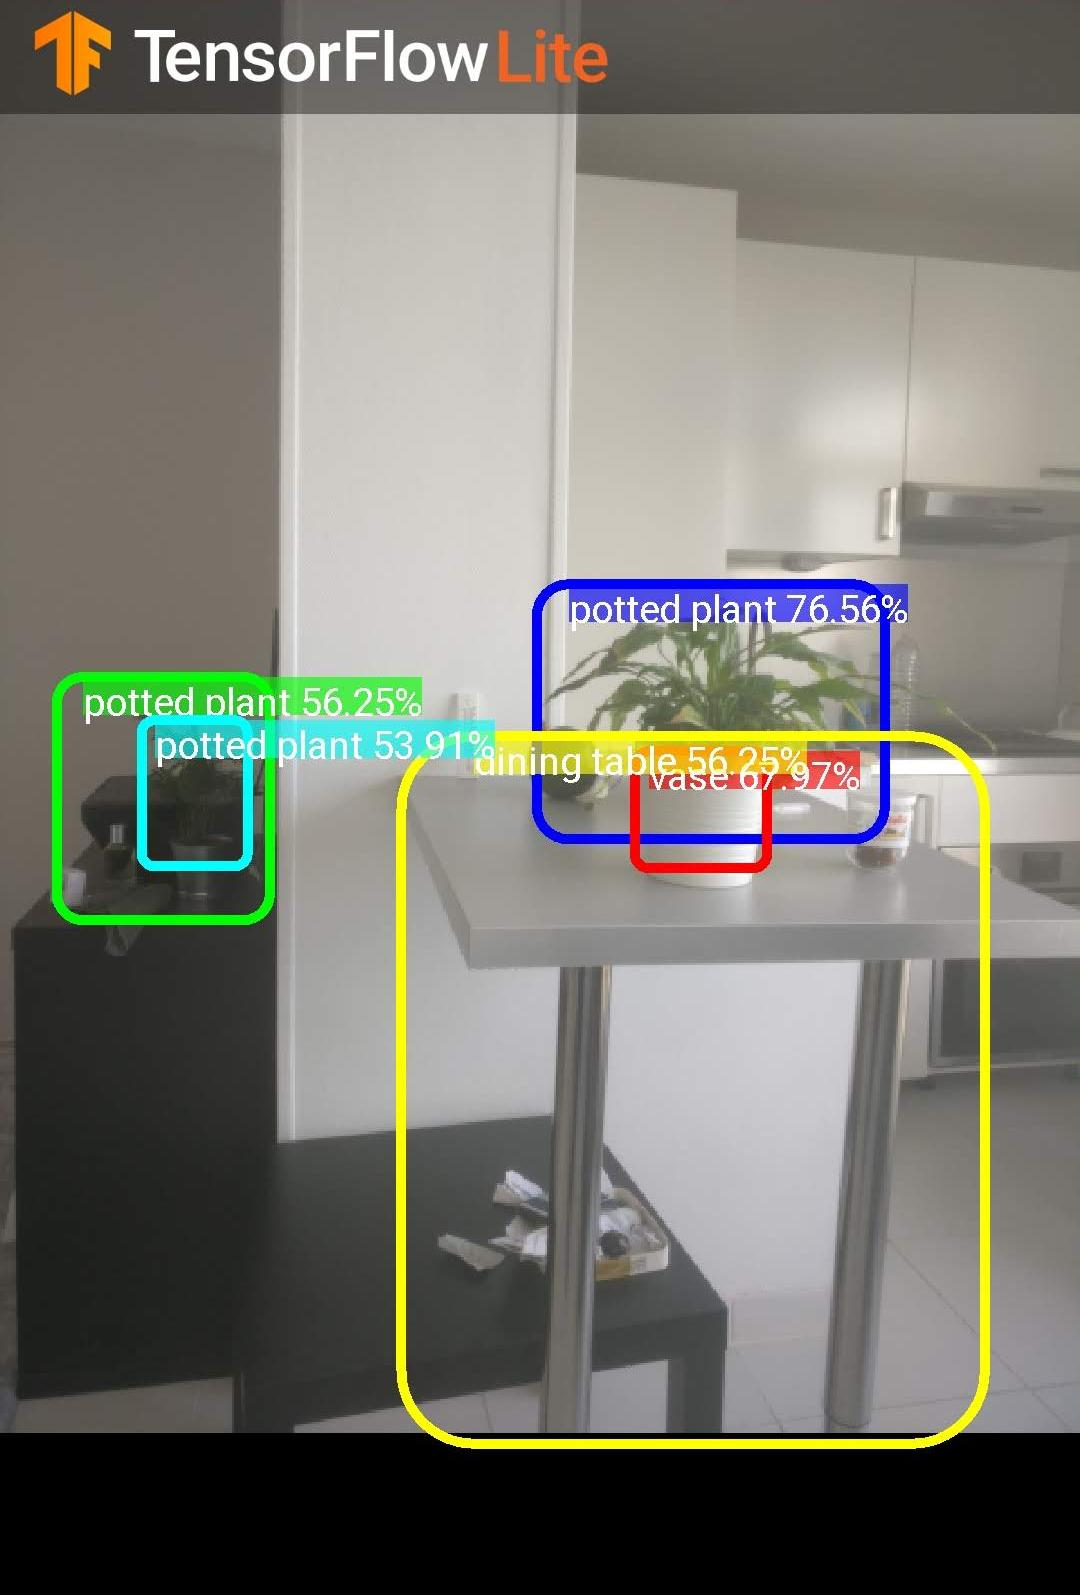
\includegraphics[width=0.7\textwidth]{images/object_detection.jpg}
  \caption{Exemple de reconnaissance d'objet}
  \label{fig:objectdetection}
\end{figure}

 Ce type de modèle (objet detection) est entraîné avec des objets de différentes classes (vêtements, fruits, etc.). Avec TensorFlow, lorsqu'on met à l'entrée de ce type de modèle une image, on obtient en sortie une liste d'objets avec chacun sa localisation, sa classe et un degré de confidence (qui correspond à la fiabilité de l'objet identifié).

\begin{figure}[h!]
\centering
  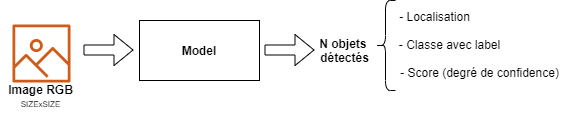
\includegraphics[width=0.7\textwidth]{images/schema_objectDetection.png}
  \caption{Schema principe de fonctionnement d'un modèle}
  \label{fig:schema_objectdetection}
\end{figure}

En revanche, les modèles de \textbf{classification} avec TensorFlow ne détecte qu'un seul élément sur une image et ne fournit pas précisément sa localisation. Ces modèles sont entraînés sur une seule classe générique (exemple : vêtements, aliments, plantes, etc.) qui va ensuite être capable d'identifier l'élément de manière plus précise. Exemple : \\

\begin{itemize}
  \item Classe vêtements : T-shirt, jean, ...
  \item Classe aliments : salade, pâtes, ...
  \item Classe fruits : pomme, banane, ...  
  \item Classe insectes : sauterelle, abeille, papillon, ...
  \item  ...
\end{itemize}

\newpage

\begin{figure}[h!]
\centering
  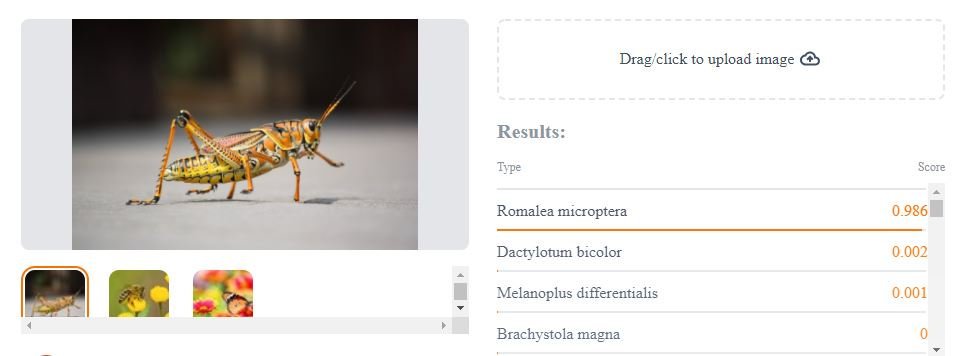
\includegraphics[width=\textwidth]{images/insects_classification.jpg}
  \caption{Exemple de classification d'insectes}
  \label{fig:insectsclassification}
\end{figure}

\subsubsection{Choix du modèle} \label{choixmodele}
Notre objectif pour notre premier prototype est d'utiliser un modèle qui reconnaît un maximum d'objet dans différentes classes. Cela permettrait donc aux utilisateurs finaux détecter un ensemble d'objet de différentes catégories plutôt que d'une seule catégorie spécifique. De ce point de vue, les modèles de classification tels qu'on les a vus précédemment ne correspondraient donc pas à ce besoin. Néanmoins, pour des versions ultérieures de l'application, il pourra être envisagé, soit une amélioration du modèle utilisé pour que celui-ci soit plus précis, ou ajouter la possibilité de changer de modèle au sein de l'application. Il nous faut donc choisir parmi les deux modèles disponibles évoqués précédemment à savoir SSD MobileNet et Mobile Object Localizer. On pourra par la suite comparer le modèle choisi parmi ces deux-là avec les autres modèles entraînés à l'aide d'autres banques d'images \footnote{\url{https://github.com/tensorflow/models/blob/master/research/object_detection/g3doc/tf1_detection_zoo.md}}. \\

Ces deux modèles permettent donc d'identifier des objets, parmi les objets connus du modèle et d'en fournir leurs positions dans l'image. Tout deux utilisent l'architecture de réseau de neurones MobileNet \footnote{\url{https://arxiv.org/abs/1801.04381}}. SSD MobileNet a été entraîné avec la banque d'image COCO dataset \footnote{\url{https://cocodataset.org/}}. Cependant, une autre version disponible uniquement sur PC a été entraîné avec Open Images V4 \footnote{\url{https://storage.googleapis.com/openimages/web/index.html}}. En revanche, aucune information sur la banque d'image utilisée pour Mobile Object Localizer.

Pour faire notre choix de modèle, il est intéressant de comparer ses deux modèles en faisant un benchmark. En effet TensorFlow dispose d'un outil qui permet de mesurer et faire des calculs de statistiques sur les modèles. L'outil permet de mesurer le temps d'initialisation du modèle, le temps de traitement (inference time), et bien d'autres données. Dans notre cas, le critère intéressant à mesurer serait la latence du modèle. Les résultats des benchmarks varient beaucoup en fonction du smartphone utilisé. Ci-dessous les résultats de benchmarks qui ont été fait par TensorFlow sur différents appareils.

\begin{figure}[h!]
\centering
  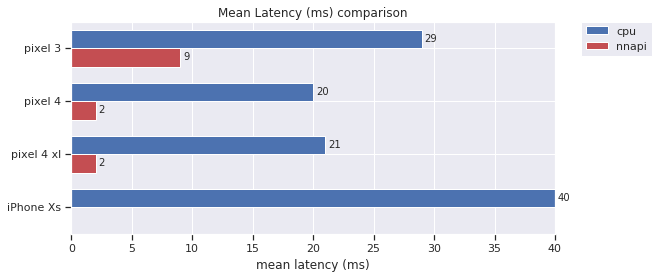
\includegraphics[width=\textwidth]{images/bench_mol.png}
  \caption{Benchmark de Mobile Object Localizer sur plusieurs appareils}
  \label{fig:benchmol}
\end{figure}

(Remarque: Ici aucune indication sur le nombre de threads utilisés)

\begin{figure}[h!]
\centering
  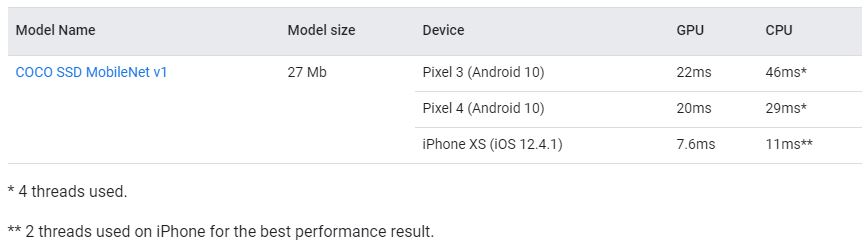
\includegraphics[width=\textwidth]{images/bench_ssd_mobilenet.jpg}
  \caption{Benchmark de SSD MobileNet sur plusieurs appareils}
  \label{fig:benchssdmobilenet}
\end{figure}

Travaillant sur le Samsung Galaxy S10e dans le cadre de ce projet, il serait plus pertinent de mesurer les performances de ces deux modèles sur ce smartphone également. Ci-dessous les résultats obtenus :
\newpage

\begin{figure}[h!]
\centering
  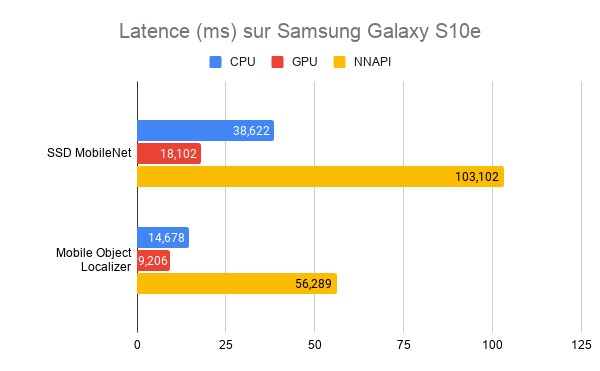
\includegraphics[width=\textwidth]{images/bench_s10e.png}
  \caption{Benchmark sur Samsung Galaxy S10e}
  \label{fig:benchs10e}
\end{figure}

Pour conclure sur ces mesures, on peut voir donc clairement que le modèle SSD MobileNet présente plus de latence que Mobile Object Localizer. Il serait donc plus judicieux de choisir ce modèle là. Cependant, pour utiliser ces modèles, nous avons besoin d'un fichier important parmi les méta-data du modèle qui est le fichier label. Ce fichier stock les labels de toutes les classes d'objets connu par le modèle. En l'abscence de ce fichier qui doit accompagner le modèle, il est donc impossible d'attribuer un label à un objet détecté. Or, le fichier accompagnant le Mobile Object Localizer est vide et aucun moyen de le retrouver ou d'extraire ces données.  On peut d'ailleurs voir directement le résultat de l'absence de données dans ce fichier sur le site \footnote{\url{https://tfhub.dev/google/lite-model/object_detection/mobile_object_localizer_v1/1/default/1}} :

\begin{figure}[h!]
\centering
  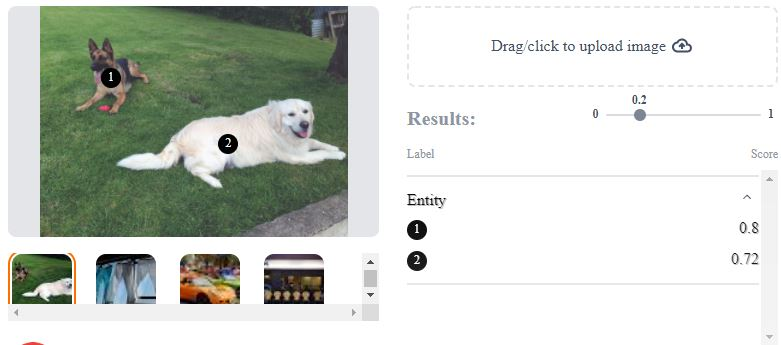
\includegraphics[width=.6\textwidth]{images/labels_empty.JPG}
  \caption{Résultat d'un labelmap vide}
  \label{fig:labelsempty}
\end{figure}

Les objets sont détectés et localisés, mais aucun label leur est assigné. Souhaitant informer l'utilisateur de l'objet détecté, nous retenons plutôt le modèle SSD MobileNet.

\subsection{Implémentation sur Android}
Pour utiliser les modèles sur Android, il existe deux solutions : \textbf{lib\_task\_api} et \textbf{lib\_interpreter}. Lib task api utilise l'API prête à l'emploi TensorFlow Lite Task Library \footnote{\url{https://www.tensorflow.org/lite/inference_with_metadata/task_library/object_detector}}. C'est une libraire qui contient un ensemble de fonction facile à utiliser pour les développeurs d'application de machine learning sur TensorFlow. Il fournit des opérations prêtes à l'emploi notamment pour manipuler les modèles et les interpréter. Lib\_interpreter se base sur l'interpréteur Java : TensorFlow Lite Interpreter API \footnote{\url{https://www.tensorflow.org/lite/guide/inference}}. Cet interpréteur Java est disponible en tant que librairie Android et on peut donc implémenter directement la classe \verb|Interpreter|.
Pour utiliser ces méthodes, il suffit des les importer à l'aide du gestionnaire de dépendance Gradle.
\begin{lstlisting}
dependencies {
    //...

    // Build off of nightly TensorFlow Lite Task Library
    implementation('org.tensorflow:tensorflow-lite-task-vision:0.0.0-nightly') { changing = true }
 }
\end{lstlisting}

L'interpreter Java quand à lui est disponible directement au niveau de \\ \verb|org.tensorflow:tensorflow-lite|.

\section{Informer l'utilisateur}
Le deuxième aspect important de ce projet est l'interaction avec l'utilisateur. Les utilisateurs finaux étant des aveugles, le programme ne pourra pas se contenter d'afficher du texte à l'écran, ou de marquer les zones où les objets ont été détectés. Il faut donc trouver un moyen pour informer l'utilisateur des données renvoyées par le système. Pour répondre à ce besoin, il est intéressant de faire un état de l'art et voir ce qui se fait sur ce genre d'application.

\subsection{Solutions existantes}
Il est important de noter que les aveugles utilisent les smartphones comme les nôtres, mais parfois en complément d'outils externes (physique) ou interne (logiciel). Parmi les outils physiques, il y a la solution proposée par la start-up française Telorion. Cette solution met en place une coque amovible en élastomère avec des perforations qui permettent aux aveugles de naviguer sur les différents menus.

\newpage

\begin{figure}[h!]
\centering
  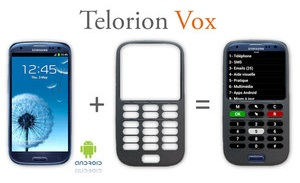
\includegraphics[width=.7\textwidth]{images/telorion_case.JPG}
  \caption{Coque amovible Telorion}
  \label{fig:telorioncase}
\end{figure}

Cette solution est accompagnée d'une couche logicielle avec le Telorion Vox et le Telerion Zoom qui permettent d'avoir un retour sonore ou faire des zooms par exemple pour les malvoyants.

Une autre solution physique est d'utiliser un clavier en braille externe connecté au téléphone. Cette solution est notamment utilisée pour faire de la saisie de texte, comme répondre à un SMS ou envoyer un mail par exemple. La saisie de texte peut aussi se faire par dictée vocale.

Aujourd'hui, la plupart des personnes aveugles utilisent plutôt des solutions exclusivement logiciel. Ces solutions se basent sur un retour sonore qui peuvent aller du simple "bip" (lors d'une gestuelle précise sur l'écran par exemple) au lecteur d'écran (comme VoiceOver sur Apple et TalkBack sur Android) ou encore des assistants vocaux comme Siri et Google Now. Ces solutions sont intéressantes, car rapide et permettent aux utilisateurs d'avoir moins de manipulations complexes.

\subsection{Synthèse vocale}
Un état des lieux des applications existantes sur le play store d'Android nous a permis de voir que beaucoup d'application pour ce type d'usage utilisent la synthèse vocale. On peut par exemple trouver des lecteurs de texte, des applications qui permettent d'identifier de la monnaie, etc. Avec la synthèse vocale, les utilisateurs ont donc un retour sonore sur le billet d'argent souhaité ou le document scanné.

Le fonctionnement au final est simple, il suffit de donner au Text-To-Speech (différent de Speech-to-Text qui est la reconnaissance vocale) le texte à lire. Il sera ensuite énoncé par la voix synthétique de l'appareil. Plusieurs paramètres peuvent être ajustés comme la voix de la synthèse vocale, la langue, ou encore la rapidité.

Pour implémenter cette solution sur Android, on peut utiliser la classe portant le même nom : TextToSpeech. Après initialialisation de l'objet, il nous suffit ensuite de lui donner le texte à lire ; dans notre cas l'objet identifié.

\newpage

\begin{lstlisting}[language=Java]
TextToSpeech tts;

tts = new TextToSpeech(this, new TextToSpeech.OnInitListener() {
        @Override
        public void onInit(int status) {
    		// Do something
        }
      });
      tts.setLanguage(Locale.US);

/**
*  Detection processing ...
*/

tts.speak(result.getTitle(), TextToSpeech.QUEUE_FLUSH, null, null);
\end{lstlisting}

\subsection{Rendre le message compréhensible}
L'application détecte les objets en temps réel et affiche les labels et les positions correspondantes de manière instantanée. Chaque frame du flux vidéo est donc soumis au traitement et donc les valeurs en sorties sont instantanément mise à jour également. Le retour sonore qui doit énoncer les objets identifiés, se répète donc plusieurs fois de manière non stop. Autre problème également est le nombre d'objet sur une image. Comment indiquer à l'utilisateur chaque objet détecté en évitant cette problématique de répétition ? Il faut donc trouver un moyen de rendre cela plus compréhensible par l'utilisateur et moins agaçant. Plusieurs solutions peuvent être mis en place pour tenter de palier à ces problèmes. Ci-dessous l'analyse de quelques-unes d'entre elles. 

\subsubsection{Meilleure gestion de la synthèse vocale}
La première solution est de jouer sur le moment où l'objet est énoncé. On peut mettre en place des conditions qui vont faire qu'on va énoncer l'objet uniquement si ces conditions sont respectées. On peut mettre par exemple une condition sur le temps entre deux énoncés. Attendre un certain délai avant de reprononcer le nom de l'objet. Cependant, avec cette condition, l'utilisateur peut avoir une sensation de latence. On peut mettre une autre condition sur l'objet. Si l'objet prononcé précédemment est le même, alors on ne le prononce pas en boucle. L'inconvénient de cette deuxième condition est que l'objet va être énoncé qu'une fois (sauf changement) et donc l'utilisateur peut ne pas avoir entendu correctement. Il devra pointer sur un autre objet puis revenir sur l'objet précédent pour entendre à nouveau.
\subsubsection{Capteurs}
Une autre solution serait d'utiliser les différents capteurs du smartphone (accéléromètre + gyroscope) afin de détecter un déplacement dans l'espace. On pourrait alors estimer que si le smartphone est immobile, alors le synthétiseur ne reprononce pas l'objet en cours. Le problème de cette solution est que malgré que le smartphone reste immobile, le flux vidéo de la caméra peut changer et d'autres objets peuvent apparaître. Ils ne seront donc pas énoncé tant que le smartphone n'aura pas bougé.
\subsubsection{Viseur}
Pour palier au problème des objets multiples sur une image, on pourrait imaginer un système de viseur central qui va permettre d'isoler l'objet au centre de l'écran. Ce sera donc uniquement cet objet-là qui sera énoncé.

\begin{figure}[h!]
\centering
  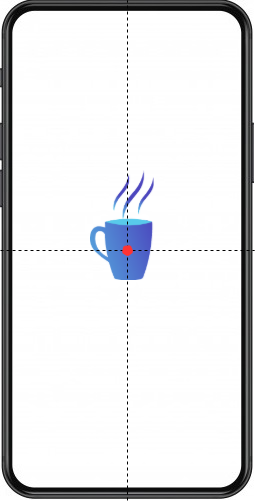
\includegraphics[width=.4\textwidth]{images/viseur.png}
  \caption{Illustration du viseur}
  \label{fig:viseur}
\end{figure}

Ensuite, pour les autres objets, on peut mettre en place d'autres solutions pour indiquer à l'utilisateur qu'il y a plusieurs objets sur l'image (par vibrement ou phrases pré-enregistrées).

\subsubsection{Vibreur}
Avec le vibreur, on peut avoir un retour permettant à l'utilisateur de savoir s'il est sur un objet ou pas. Ce sera donc une action de confirmation, combiné avec le viseur, qui dès lors que le viseur est sur un objet, le vibreur est enclenché. Si le viseur est plutôt une zone au centre de l'écran et non un point, on pourrait faire vibrer le téléphone lorsque l'objet entre dans cette zone. Ensuite, si l'objet se retrouve au centre, on cite son nom.
Autre fonctionnement serait d'utiliser le vibreur pour indiquer le nombre d'objet détecté. Faire des vibrations de courte durée répétitive indiquant le nombre d'objets. Cette solution est interessante, mais une des problèmes serait le fait qu'on ne peut pas distinguer une série de vibrations avec une autre (ex: trois vibrations pour trois objets, puis quatre vibrations pour quatre objets quelques secondes après car l'utilisateur a visé ailleurs).

\subsubsection{Phrases pré-enregistrés}
Pour gérer le nombre d'objets sur une image avec la synthèse vocale, on pourrait indiquer à l'utilisateur directement le nombre d'objets présents. Le synthétiseur lira une phrase pré-enregistrés avec le nombre d'objets présents mis à jour à chaque fois (ex: "trois objets détectés"). Cette solution reste intéressante mais peut présenter un inconvénient en terme de rapidité de restitution de l'information en cours. Pour limiter cela, on peut envisager de mettre juste des mots plutôt qu'une phrase complète. Couplé à la solution du viseur présenté plus haut, on peut indiquer ou se situe l'objet par rapport au viseur si l'utilisateur n'arrive pas à le viser (le mettre au centre). On peut indiquer "gauche" ou "haut", etc. pour dire plus précisément où se situe l'objet.

\section{Navigation}
\textbf{(En cours... À venir sur les prochaines versions du CDA)}
\subsection{Guide d'utilisation}
//guide première utilisation...
\subsection{Accès aux réglages}
//reglage vitesse synthétiseur, reglage mode...

\annexes

\end{document}